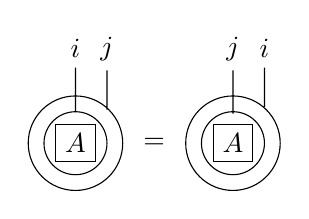
\begin{tikzpicture}
    \coordinate(origin1)at(0,0);
    \coordinate(origin2)at(2,0);
    \node at(0,1.2)[anchor=center](i1){$i$};
    \node at(.4,1.2)[anchor=center](j1){$j$};
    \node at(2.4,1.2)[anchor=center](i2){$i$};
    \node at(2.,1.2)[anchor=center](j2){$j$};
    \draw
    (origin1) node[anchor=center, draw, rectangle](A1){$A$}
    (i1.south)--++(0,-.55)
    (j1.south)--++(0,-.5)
    (A1.center) circle[radius=.4]
    (A1.center) circle[radius=.6]
    ;
    \draw
    (origin2) node[anchor=center, draw, rectangle](A2){$A$}
    (i2.south)--++(0,-.5)
    (j2.south)--++(0,-.55)
    (A2.center) circle[radius=.4]
    (A2.center) circle[radius=.6]
    ;
    \node[anchor=center]at(1,0){$=$};
\end{tikzpicture}
